\section{Boundary condition in dissipative particle dynamics}


\subsection{模型}
\frame{\frametitle{模型}
\begin{columns}
\begin{column}[c]{0.4\textwidth}
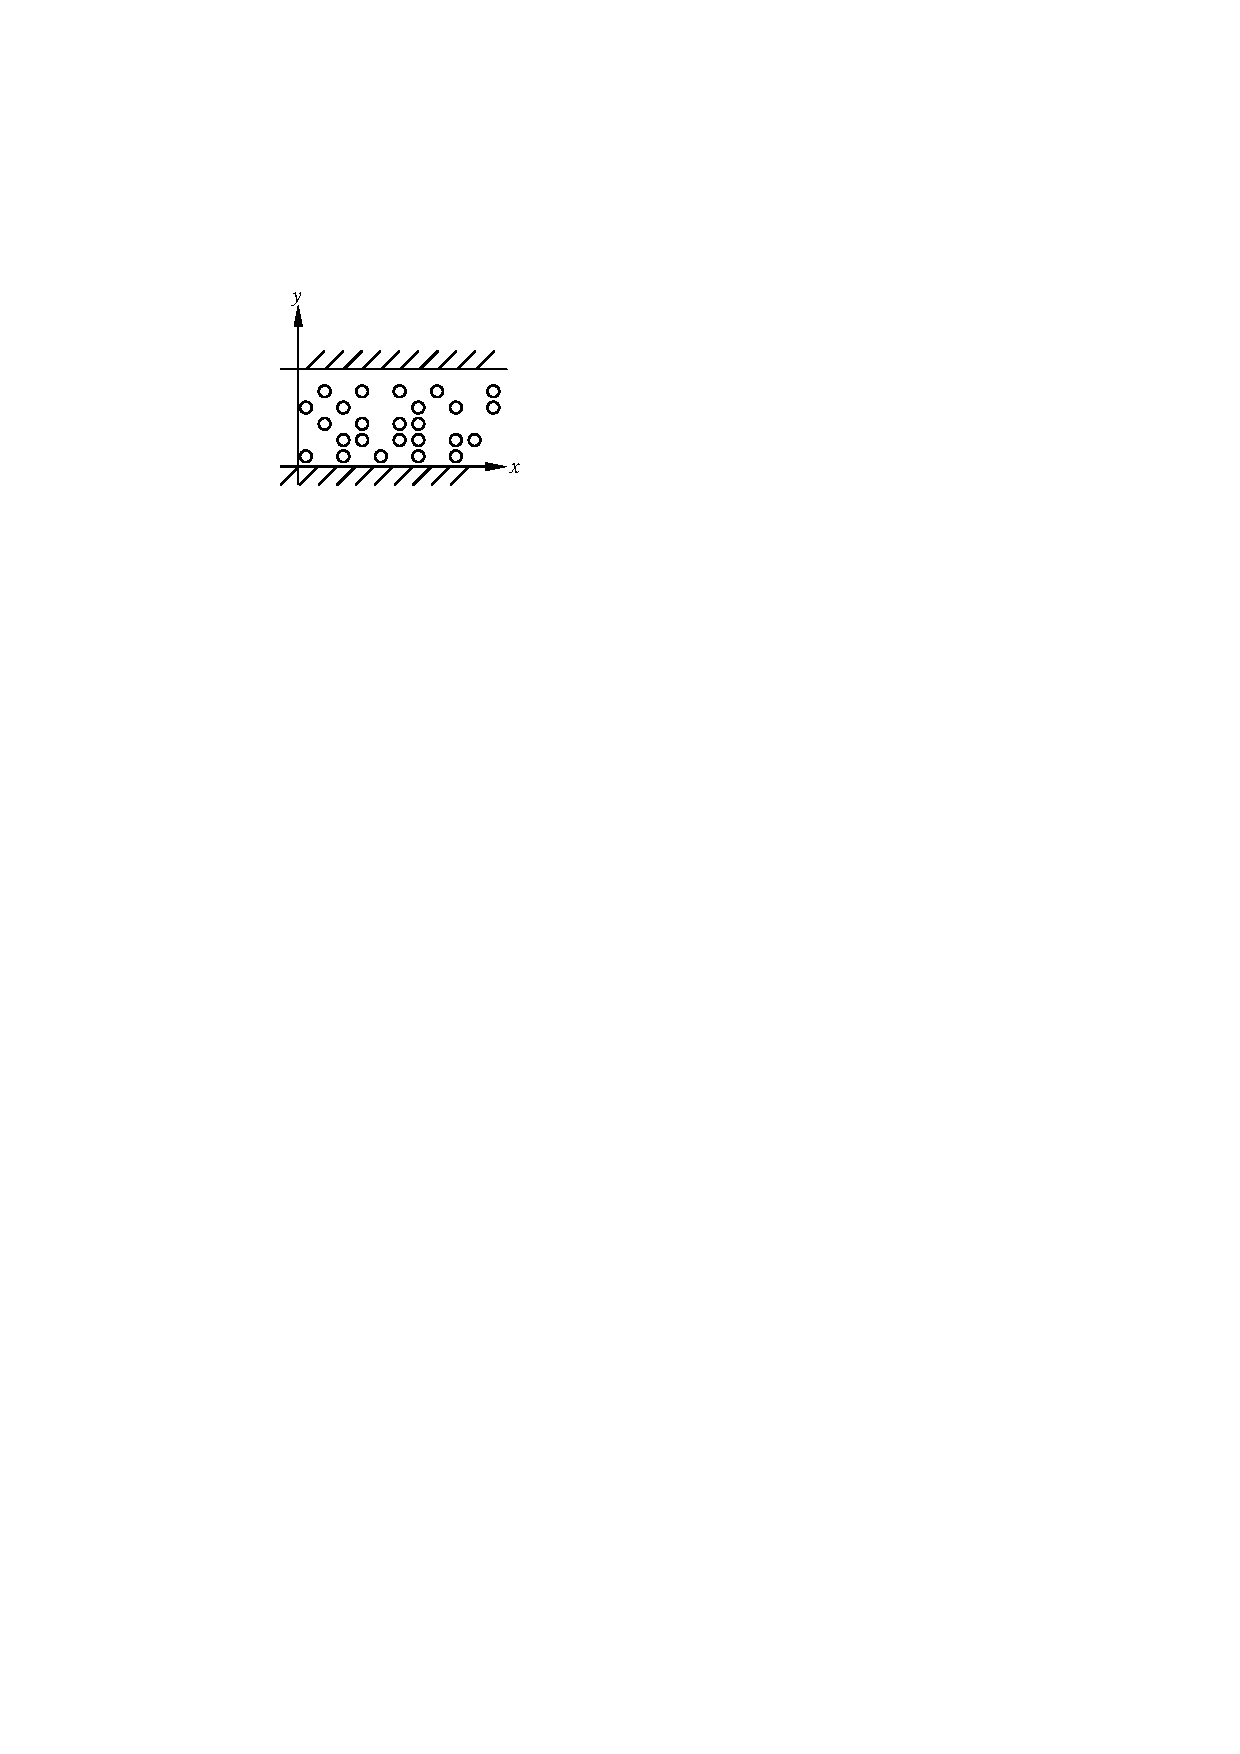
\includegraphics[width=1\textwidth]{./figures/fig04.pdf}

这篇文章对上图的模型分别对反弹映像的三种边界条件作了研究.
\end{column}
\begin{column}[c]{0.6\textwidth}

Dimensionless friction coefficient:
\[
\tau = \gamma\lambda/dv_T
\]

$\gamma$: friction coefficient. $\lambda$: average distance between particles. $d$: spatial dimension(=2). $v_T=\sqrt{k_bT/m}$

The two components of temperature:
\[
T^x = \sum_im_iv_{x_i}^2
,T^y = \sum_im_iv_{y_i}^2
\]
\end{column}
\end{columns}
}

\subsection{结果}
\frame{\frametitle{结果}

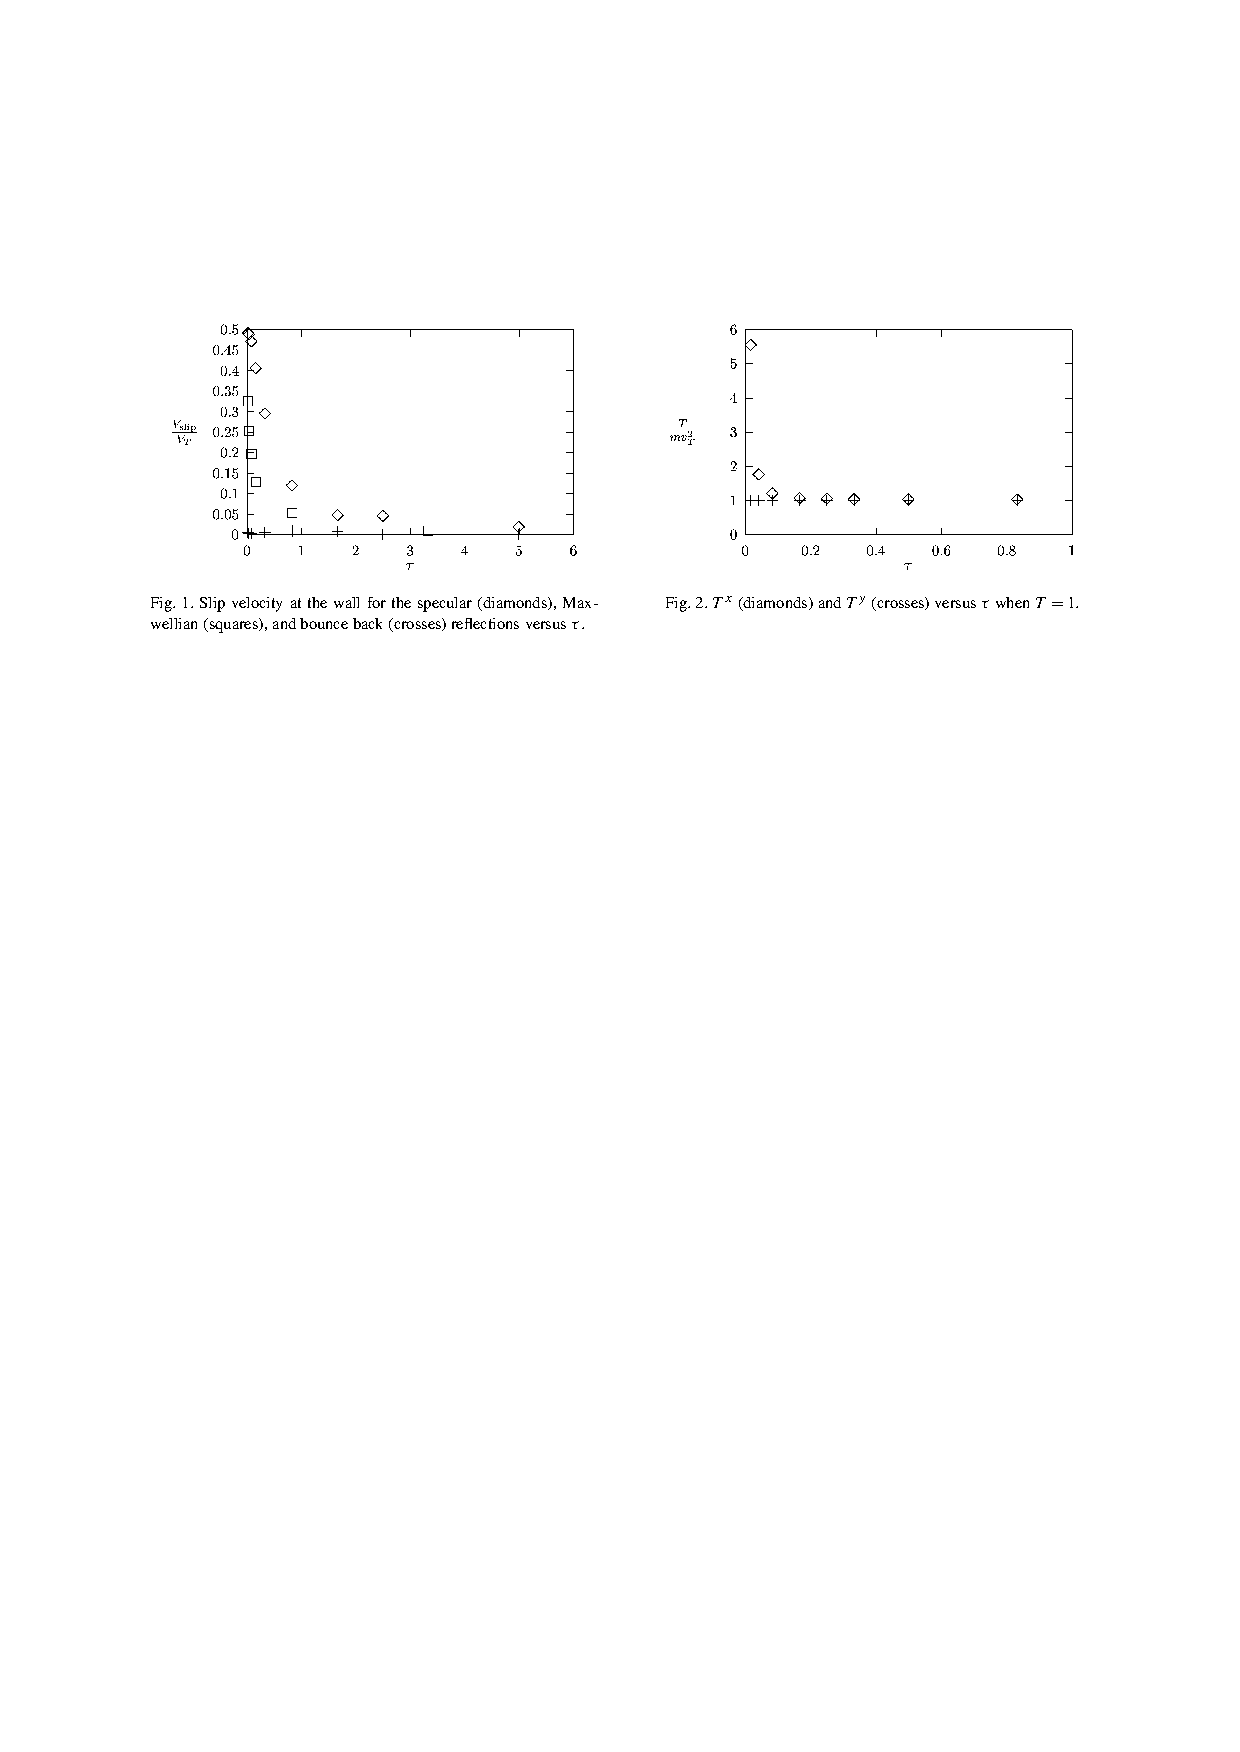
\includegraphics[width=1\textwidth]{./figures/fig05.pdf}
}

